% directive: parallelReedSolomonFigure
% aria-label: Parallel Reed-Solomon encoding: each message chunk m_i has 16 coordinates m_i[0], ..., m_i[15]; each row l is encoded by its own polynomial P_l with P_l(x_i) = m_i[l]; the columns of the resulting 16 by N grid are the chunks Encode(m, j).
\documentclass[tikz,border=6pt]{standalone}
\usepackage[T1]{fontenc}
\usepackage{amsmath,amssymb}
\renewcommand{\familydefault}{\sfdefault}
\usepackage[eulergreek]{sansmath}
\sansmath
\usepackage{xcolor}
\usepackage{tikz}
\usetikzlibrary{positioning,calc,arrows.meta,fit,backgrounds,decorations.pathreplacing}
\definecolor{commentcolor}{HTML}{666666}
\definecolor{signalblue}{HTML}{3A76F0}
\definecolor{signalgreen}{HTML}{2A7B7B}
\definecolor{signalolive}{HTML}{4E7F60}
\definecolor{signalpurple}{HTML}{6B3FA0}
\definecolor{adversaryred}{HTML}{B42318}
\newcommand{\Encode}{\mathsf{Encode}}
\newcommand{\Decode}{\mathsf{Decode}}
\tikzset{
  panel/.style={draw=gray!45, line width=0.5pt, rounded corners=4pt, fill=gray!3, inner sep=6pt},
  algbox/.style={draw=signalolive!80, line width=0.7pt, rounded corners=3pt, fill=signalolive!10,
    inner sep=6pt, font=\small\sffamily, align=center},
  statebox/.style={draw=signalblue!70, line width=0.65pt, rounded corners=4pt, fill=signalblue!6,
    inner sep=6pt, font=\small\sffamily, align=center},
  keypill/.style={draw=signalpurple!75, line width=0.6pt, rounded corners=7pt, fill=signalpurple!9,
    inner xsep=8pt, inner ysep=4pt, font=\small\sffamily},
  chunk/.style={draw=signalblue!75, line width=0.55pt, rounded corners=2pt, fill=signalblue!9,
    minimum width=0.62cm, minimum height=0.50cm, inner sep=1pt, font=\scriptsize\sffamily},
  chunklost/.style={chunk, draw=gray!45, fill=gray!10, text=gray!55},
  sourcechunk/.style={chunk, draw=signalpurple!70, fill=signalpurple!9},
  goodpill/.style={draw=signalgreen!80, line width=0.65pt, rounded corners=7pt, fill=signalgreen!9,
    inner xsep=8pt, inner ysep=4pt, font=\small\sffamily},
  failpill/.style={draw=adversaryred!75, line width=0.65pt, rounded corners=7pt, fill=adversaryred!7,
    inner xsep=8pt, inner ysep=4pt, font=\small\sffamily},
  flow/.style={->, >=Stealth, line width=0.8pt, black},
  lossy/.style={->, >=Stealth, line width=0.5pt, gray!55, dashed},
  slot/.style={draw=gray!60, line width=0.5pt, minimum width=0.42cm, minimum height=0.42cm, inner sep=0pt},
  slotfull/.style={slot, fill=signalgreen!25, draw=signalgreen!70},
  slotempty/.style={slot, fill=white},
  lbl/.style={font=\small\sffamily, inner sep=2pt},
  slbl/.style={font=\scriptsize\sffamily, inner sep=1.5pt},
  note/.style={font=\scriptsize\sffamily\itshape, text=commentcolor, inner sep=1.5pt},
  theorybox/.style={draw=signalgreen!80, line width=0.8pt, rounded corners=4pt, fill=signalgreen!8,
    inner sep=7pt, font=\small\sffamily, align=center},
  instancebox/.style={draw=signalblue!70, line width=0.7pt, rounded corners=4pt, fill=signalblue!6,
    inner sep=7pt, font=\small\sffamily, align=center},
  instof/.style={->, >=Stealth, line width=0.8pt, black},
  uses/.style={->, >=Stealth, line width=0.7pt, dashed, signalolive},
  ecbox/.style={draw=signalblue!70, line width=0.7pt, rounded corners=3pt, fill=signalblue!7,
    inner sep=6pt, font=\small\sffamily, align=center},
  rolepill/.style={fill=signalgreen, text=white, rounded corners=5pt, inner xsep=9pt, inner ysep=4pt,
    font=\sffamily\bfseries},
  advpill/.style={draw=adversaryred!80, line width=0.7pt, rounded corners=5pt, fill=adversaryred!7,
    text=adversaryred, minimum width=1.05cm, minimum height=0.68cm, inner sep=3pt, font=\normalsize},
  timeline/.style={-, line width=0.6pt, gray!55},
}
\newcommand{\tagsf}[1]{{\scriptsize\sffamily\itshape\textcolor{commentcolor}{#1}}}
\newcommand{\notesf}[1]{{\scriptsize\sffamily\itshape\textcolor{signalpurple}{#1}}}

\begin{document}
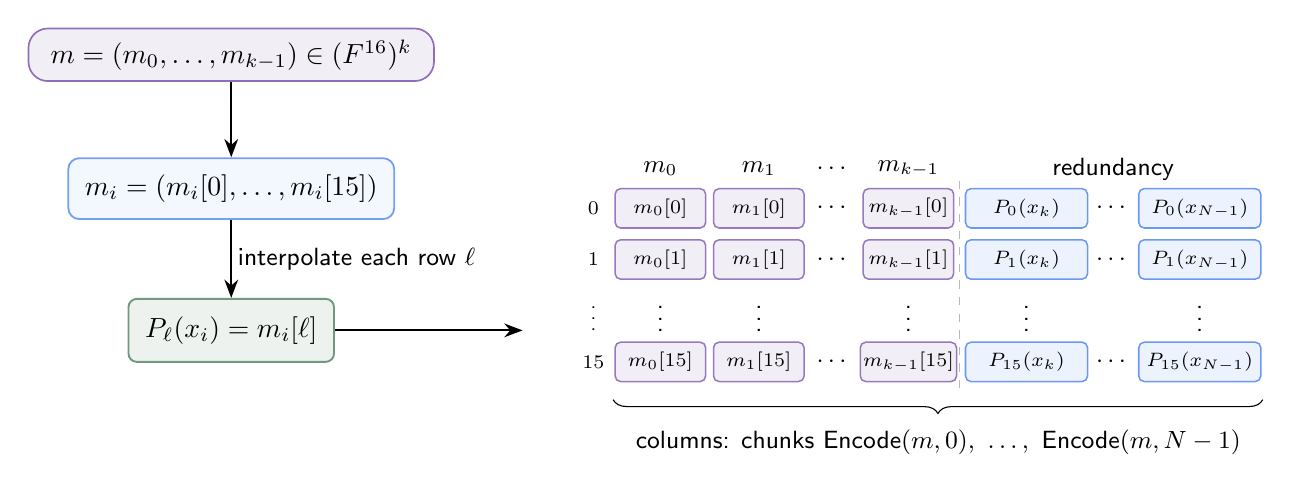
\begin{tikzpicture}[x=1cm,y=1cm]
  \node[keypill, font=\normalsize] at (-5.95,2.25) (msgin) {$m=(m_0,\ldots,m_{k-1})\in(F^{16})^k$};
  \node[statebox, minimum width=3.40cm, font=\normalsize] at (-5.95,0.55) (tuplein)
    {$m_i=(m_i[0],\ldots,m_i[15])$};
  \node[algbox, minimum width=2.60cm, minimum height=0.80cm, font=\normalsize] at (-5.95,-1.25) (poly)
    {$P_\ell(x_i)=m_i[\ell]$};
  \draw[flow] (msgin.south) -- (tuplein.north);
  \draw[flow] (tuplein.south) -- node[midway, right, lbl] {interpolate each row $\ell$} (poly.north);
  \draw[flow] (poly.east) -- (-2.25,-1.25);
  \begin{scope}[shift={(2.2,-1.25)}]
  \node[slbl, font=\small\sffamily] at (-2.70,2.05) {$m_0$};
  \node[slbl, font=\small\sffamily] at (-1.45,2.05) {$m_1$};
  \node[slbl, font=\small\sffamily] at (-0.50,2.05) {$\cdots$};
  \node[slbl, font=\small\sffamily] at (0.45,2.05) {$m_{k-1}$};
  \node[slbl, font=\small\sffamily] at (3.05,2.05) {redundancy};
  \node[slbl] at (-3.55,1.55) {$0$};
  \node[slbl] at (-3.55,0.90) {$1$};
  \node[slbl] at (-3.55,0.25) {$\vdots$};
  \node[slbl] at (-3.55,-0.40) {$15$};
  \foreach \x/\i in {-2.70/0, -1.45/1, 0.45/{k-1}} {
    \node[sourcechunk, minimum width=1.15cm] at (\x,1.55) {$m_{\i}[0]$};
    \node[sourcechunk, minimum width=1.15cm] at (\x,0.90) {$m_{\i}[1]$};
    \node[font=\small] at (\x,0.25) {$\vdots$};
    \node[sourcechunk, minimum width=1.15cm] at (\x,-0.40) {$m_{\i}[15]$};
  }
  \foreach \y in {1.55, 0.90, -0.40} {
    \node[font=\small] at (-0.50,\y) {$\cdots$};
    \node[font=\small] at (3.05,\y) {$\cdots$};
  }
  \foreach \x/\j in {1.95/{k}, 4.15/{N-1}} {
    \node[chunk, minimum width=1.55cm] at (\x,1.55) {$P_{0}(x_{\j})$};
    \node[chunk, minimum width=1.55cm] at (\x,0.90) {$P_{1}(x_{\j})$};
    \node[font=\small] at (\x,0.25) {$\vdots$};
    \node[chunk, minimum width=1.55cm] at (\x,-0.40) {$P_{15}(x_{\j})$};
  }
  \draw[gray!55, line width=0.5pt, dashed] (1.10,1.90) -- (1.10,-0.75);
  \draw[decorate, decoration={brace, mirror, amplitude=5pt}] (-3.30,-0.88) -- (4.95,-0.88);
  \node[anchor=north, font=\small\sffamily] at (0.83,-1.14)
    {columns: chunks $\Encode(m,0),\ \ldots,\ \Encode(m,N-1)$};
  \end{scope}
\end{tikzpicture}
\end{document}
